\documentclass[14pt]{extbook}
\usepackage{multicol, enumerate, enumitem, hyperref, color, soul, setspace, parskip, fancyhdr} %General Packages
\usepackage{amssymb, amsthm, amsmath, latexsym, units, mathtools} %Math Packages
\everymath{\displaystyle} %All math in Display Style
% Packages with additional options
\usepackage[headsep=0.5cm,headheight=12pt, left=1 in,right= 1 in,top= 1 in,bottom= 1 in]{geometry}
\usepackage[usenames,dvipsnames]{xcolor}
\usepackage{dashrule}  % Package to use the command below to create lines between items
\newcommand{\litem}[1]{\item#1\hspace*{-1cm}\rule{\textwidth}{0.4pt}}
\pagestyle{fancy}
\lhead{Module12L}
\chead{}
\rhead{Version B}
\lfoot{6131-5778}
\cfoot{}
\rfoot{test}
\begin{document}

\begin{enumerate}
\item{
Determine the horizontal and/or oblique asymptotes in the rational function below.\[ f(x) = \frac{9x^{3} -9 x^{2} -88 x -80}{6x^{3} + x^{2} +8 x + 80} \]} \newpage
\item{
Determine the horizontal and/or oblique asymptotes in the rational function below.\[ f(x) = \frac{20x^{3} -33 x^{2} -2 x + 15}{20x^{3} -62 x^{2} +52 x -15} \]} \newpage
\item{
Determine the vertical asymptotes and holes in the rational function below.\[ f(x) = \frac{8x^{3} -10 x^{2} -9 x + 9}{6x^{2} -5 x -6} \]} \newpage
\item{
Write an equation of a function that \textit{could} be represented by the graph below. Explain why your function could represent the graph.
\begin{center}
    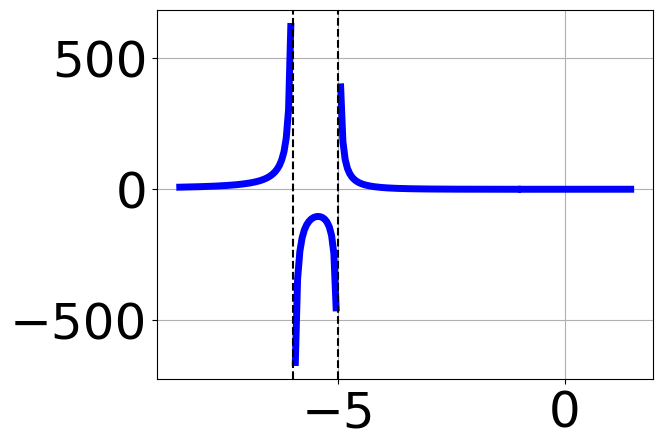
\includegraphics[width=0.5\textwidth]{../Figures/identifyGraphOfRationalFunctionB.png}
\end{center}
} \newpage
\item{
Write an equation of a function that \textit{could} be represented by the graph below. Explain why your function could represent the graph.
\begin{center}
    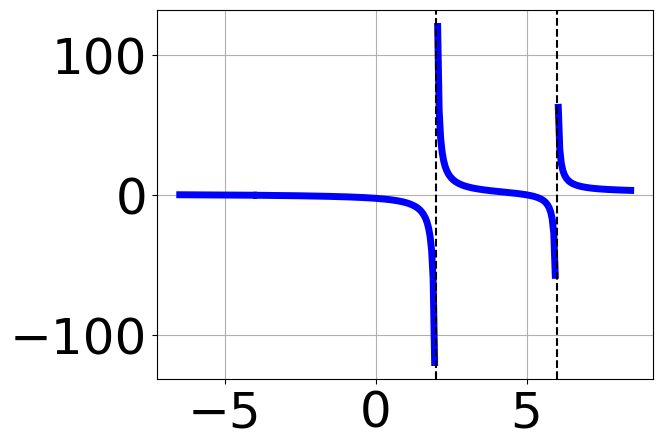
\includegraphics[width=0.5\textwidth]{../Figures/identifyGraphOfRationalFunctionCopyB.png}
\end{center}
} \newpage
\item{
Determine the horizontal and/or oblique asymptotes in the rational function below.\[ f(x) = \frac{8x^{3} -10 x^{2} -73 x -60}{4x^{2} +21 x + 20} \]} \newpage
\item{
Determine the vertical asymptotes and holes in the rational function below.\[ f(x) = \frac{12x^{3} -47 x^{2} +60 x -25}{9x^{2} -27 x + 20} \]} \newpage
\item{
Determine the vertical asymptotes and holes in the rational function below.\[ f(x) = \frac{9x^{3} +36 x^{2} -25 x -100}{12x^{2} +29 x + 15} \]} \newpage
\item{
Determine the vertical asymptotes and holes in the rational function below.\[ f(x) = \frac{8x^{3} -46 x^{2} +81 x -45}{16x^{2} -25} \]} \newpage
\item{
Determine the horizontal and/or oblique asymptotes in the rational function below.\[ f(x) = \frac{6x^{3} -35 x^{2} +34 x + 40}{3x^{2} +17 x + 10} \]} \newpage
\end{enumerate}

\end{document}